% Activate the following line by filling in the right side. If for example the name of the root file is Main.tex, write
% "...root = Main.tex" if the chapter file is in the same directory, and "...root = ../Main.tex" if the chapter is in a subdirectory.
 
%!TEX root =  testMain.tex

\chapter[Robberies in ``real'' locations]{Robberies}

In the previous chapters, we moved from a non-spatial simulation, to a very simple spatial simulation. In the simple spatial simulations, agents move through an environment, but that environment is very trivial - there are two houses, that is about it. A simulation with non-trivial environment might lead to more uncertainty, and require more interesting agent-behaviours that might prove challenging for the Bayesian Network. Additionally, by implementing non-trivial environments, we move closer to the state-of-the-art agent models for modelling crime cases.


Research questions for this chapter:

\begin{itemize}
\item Can we create a simulation that somewhat reflects a real world location?
\item Can we create an automatic BN from this simulation that fulfils the criteria we set out for it?
\end{itemize}



\section{Introduction}
We take the theme of the robbery from last chapter, and make it a street robbery. Two agents are walking around at the Grote Markt (the central town square in Groningen). One of the agents is always old, and always has a valuable object with them. This is the victim agent. The other agent is the thief, who is young, and always wants to steal the valuable object. If the thief sees the potential victim, they decide whether the potential victim is vulnerable (here: old), enough to target, and if the object is worth it. If these factors are both present, the agent will have a motive to steal, will attempt to sneak up on the victim, and rob them.

\section{Methods}

We wrote a method to convert screenshots of maps into an agent-readable environment. The maps were screenshotted from \url{http://maps.stamen.com/terrain/#18/53.21618/6.57225} and converted into greyscale. Then, they were transformed into a grid of a given size. The average greyscale value of each cell in the grid was taken and coded as either `accessible' or `non-accessible'. On the greyscale map, the color of the buildings was in the range of (189, 199) - cells within this range were coded as `inaccessible', since agents cannot walk through buildings. All other cells were `accessible'. This resulted in a map shared by all agents that constrained their movements. There are 8 cameras placed randomly on the `accessible' cells on the map, each with a visual radius of 15. Additionally, we used this map to calculate the sight lines of both cameras and agents. An agent or a camera cannot see another agent if there is an `inaccessible' grid cell on the sight line between the two.

The agents have some other features than before. Every agent has an age, to determine whether they are vulnerable or not - old people are considered more vulnerable. Every agent also has an object of a certain value, the thief's object has a value of -1, and the other agent's object has a value of 1000, to make it a tempting target. An agent decides if it wants to steal something by making a very simple risk-calculation based on their risk threshold: if the object is more expensive than their risk threshold, they will attempt to steal it (contributing to `motive'). Every agent also has a goal state, this is the location at the edge of the map. When they enter their goal state, they are essentially removed from the simulation, as they leave the relevant area. Every simulation was run for 100 timesteps, or until both agents are in their goal states. The simulation itself was ran 2500 iterations. The behaviour of the agents is shown in Figure~\ref{behaviourGM}. Agents are placed randomly on the map.


The operationalisation of the random variables is described below:
\begin{description}


\item[seen\_1\_0  ] if the victim agent is in the line of sight of the thief agent.
\item[know\_valuable\_1\_0 ] if the value is higher than the risk threshold.
\item[know\_vulnerable\_1\_0  ] if the victim's age is older than the thief's threshold age.
\item[motive\_1\_0 ] if the object is more valuable than the risk threshold, the victim's age is older than the thief's threshold age, and the thief is not already stealing from someone else. 
\item[sneak\_1\_0 ] if the thief has targeted the victim (has a motive) , but is not yet in the same position.
\item[stealing\_1\_0 ] if the thief has targeted the victim, the object's value is greater than the risk threshold, and the thief's position is the same as the victim's position. 
\item[object\_dropped\_accidentally\_0 ] at every epoch, there is a 1/500 probability that the victim agent will drop the object by accident.
\item[E\_psych\_report\_1\_0 ] if the thief has a motive, we draw an estimated risk threshold and an estimated age threshold from two normal distributions (mean = victim age, sd = 20), (mean = value good, sd = 100). If the victim is older than the thief's minimal age threshold, and the object more valuable, we estimate that the psych profile states that the victim fits the thief's profile, else not.
\item[E\_camera\_1 ] the thief is seen on any one of the cameras.
\item[E\_object\_gone\_0 ] if the object is dropped accidentally, or if the object has been stolen.
\item[E\_camera\_sees\_object\_1\_0 ]  if any camera sees the thief, and the thief has stolen the object, there is a 9\% probability at every epoch that the thief is holding the stolen object in view of the camera.

\end{description}


\begin{figure}[htbp]
\begin{center}
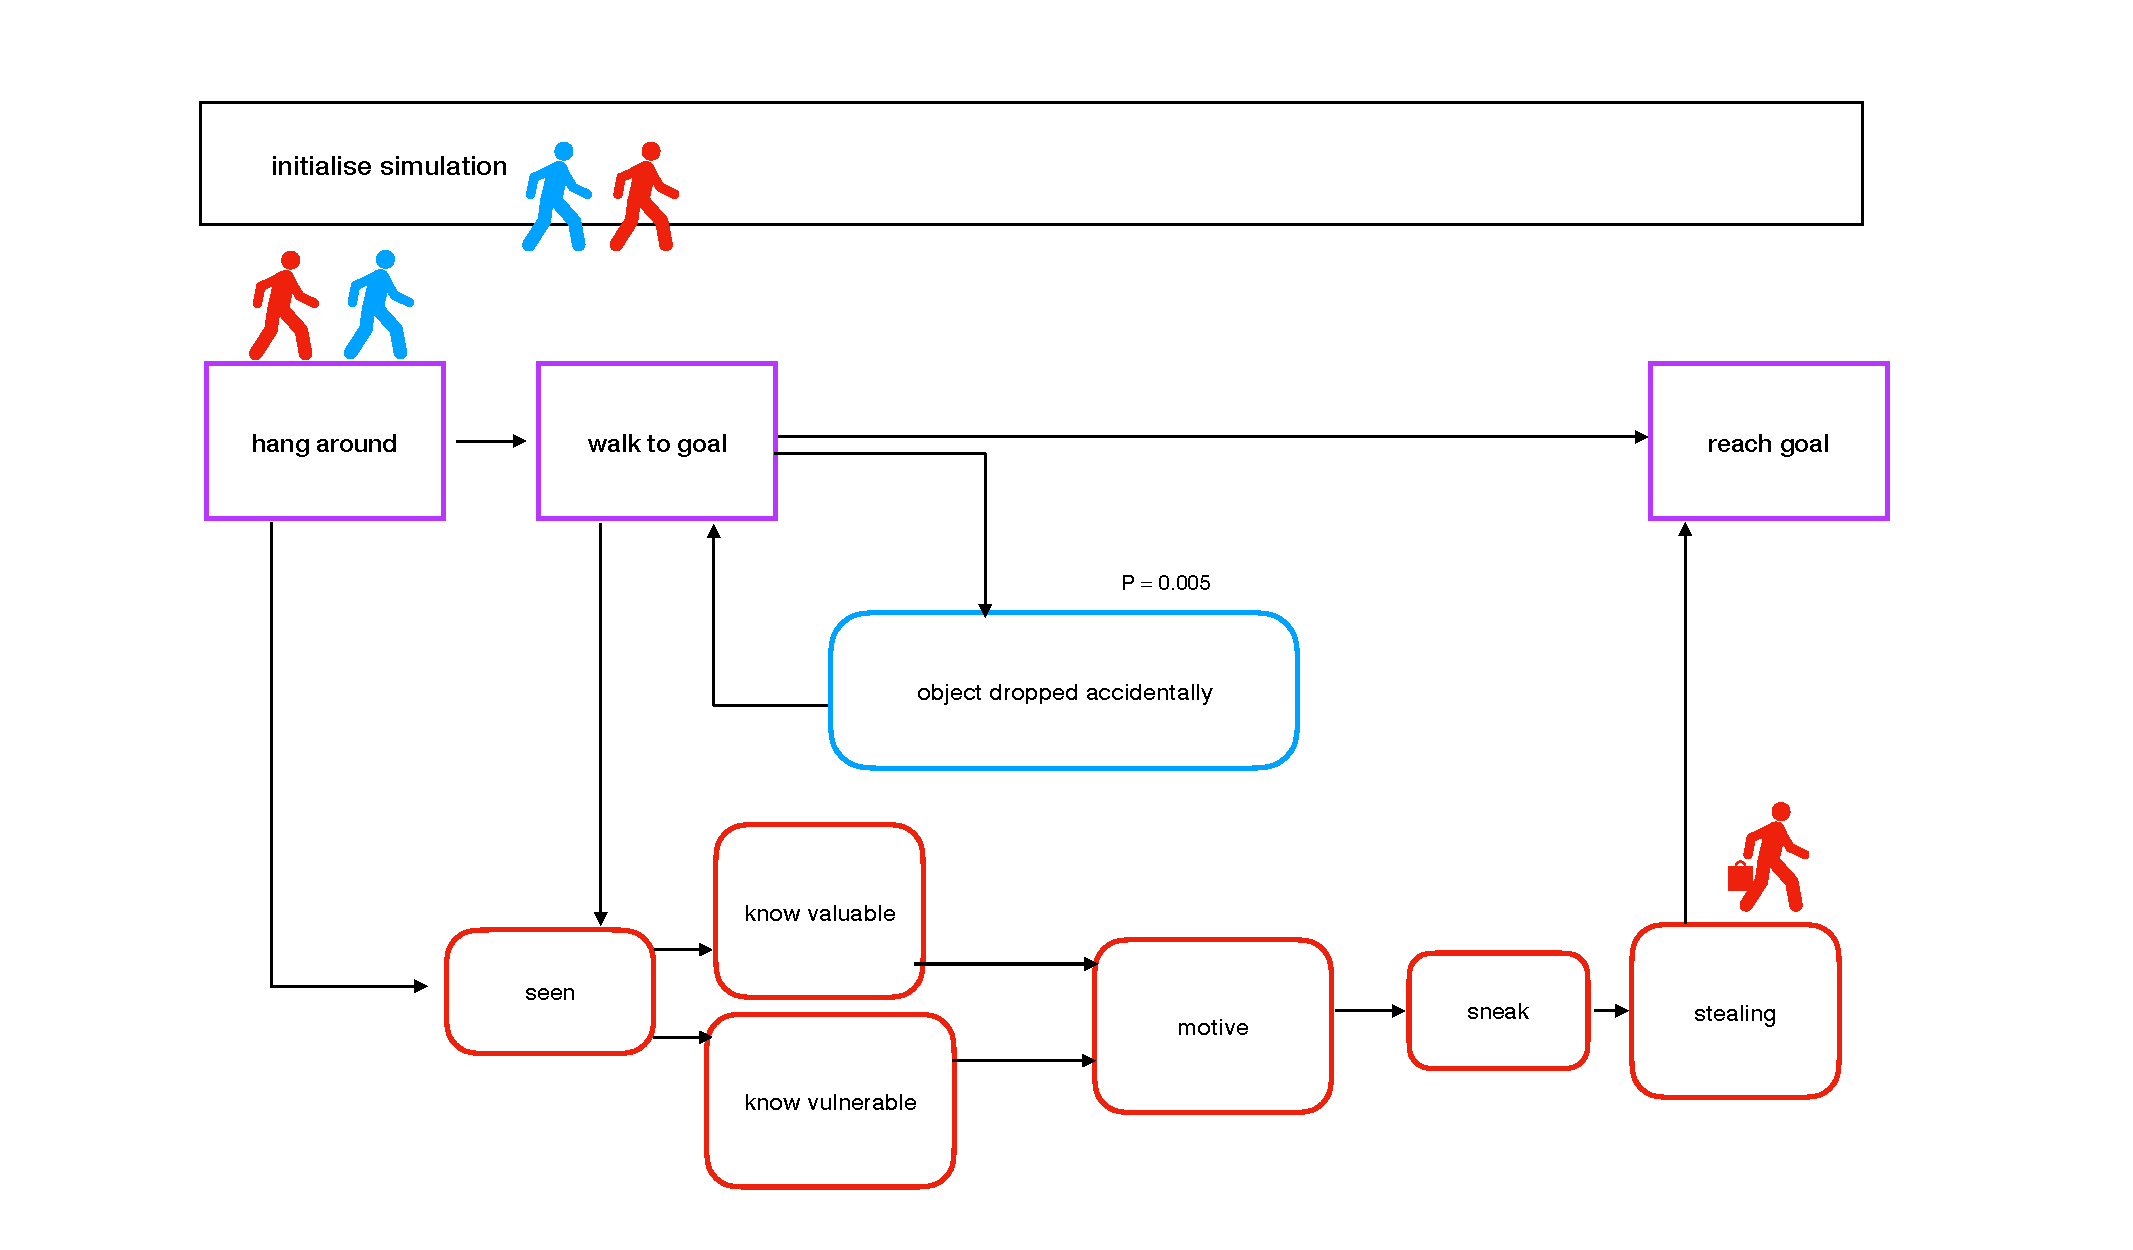
\includegraphics[width=\linewidth]{images/grotemarkt.pdf}
\end{center}
\caption{The behaviour of the agents. The nodes with rounded edges correspond to the nodes in the Bayesian Network.}
\label{behaviourGM}
\end{figure}




\begin{figure}[htbp]
\begin{center}
\begin{subfigure}{.5\textwidth}
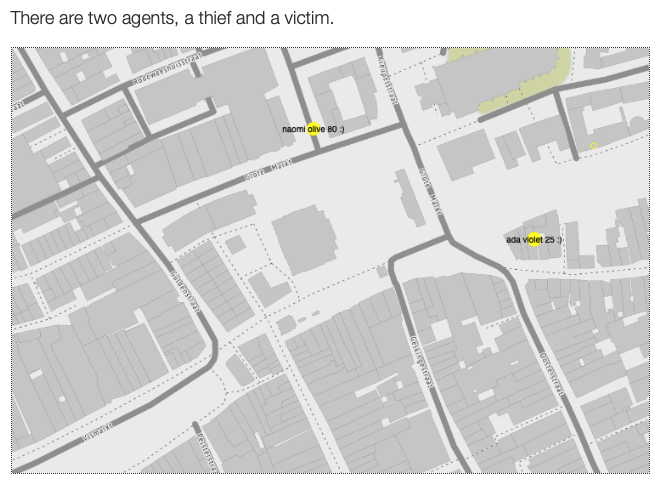
\includegraphics[width=\linewidth]{images/grotemarktmap.png}
\caption{map of environment - 2 agents}
\end{subfigure}%
\begin{subfigure}{.5\textwidth}
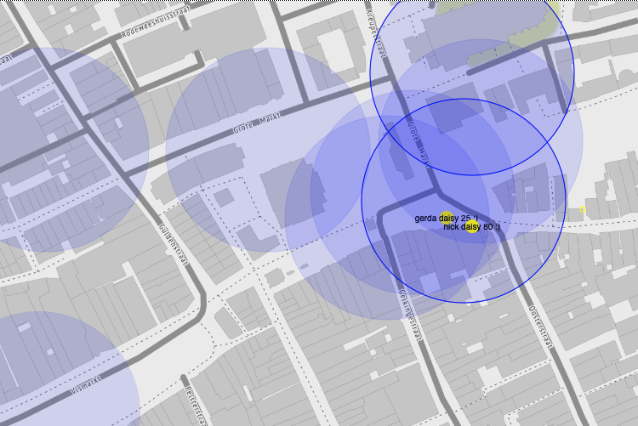
\includegraphics[width=\linewidth]{images/grotemarktCameras.png}
\caption{Camera locations are randomly initialized}
\end{subfigure}%
\label{groteMarkt}
\caption{The Grote Markt environment}
\end{center}
\end{figure}



\section{Results}

The network is shown in Figure~\ref{gmNetwork}.
\begin{figure}[htbp]
\begin{center}
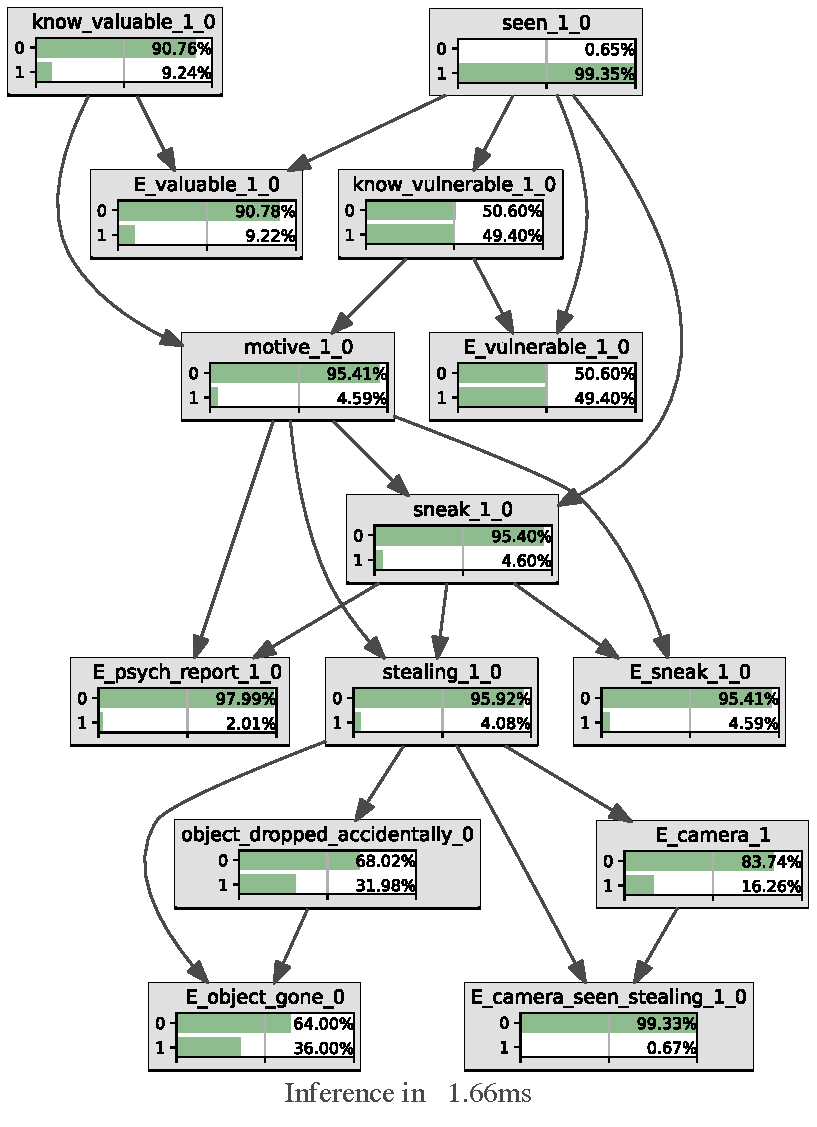
\includegraphics[width=.7\linewidth]{../experiments/GroteMarkt/bnImage/BNIMAGEGroteMarkt.pdf}
\end{center}
\caption{Bayesian Network}
\label{gmNetwork}
\end{figure}

\subsection{Structural Criteria}
\begin{enumerate}
\item \textbf{ Hypotheses are ordered temporally. }

Due to the ordering as presented to the K2 algorithm, we see that most of the hypotheses nodes from the main scenario are ordered temporally. The node `object\_dropped\_accidentally\_0' is the one exception. This node represents the alternative scenario where the thief does not steal, but the victim agent drops their object by accident. When the two scenarios are merged when the ordering is presented to the K2 algorithm, the second scenario is added after the first scenario, but before the evidence, because the second scenario occurs less frequently. It is correct that the node is connected to the `motive\_1\_0'  and `stealing\_1\_0' nodes, because the thief cannot have a motive or steal an object of the victim if the victim does not possess the object anymore. Ideally, we would want this node to have no parents. That this does not happen is a flaw in the naive calculation of the temporal ordering - we should not just look at ordering, but at the time-step of the event instead to produce correct temporal ordering of merged scenarios.

\item \textbf{Evidence connects to hypotheses.}

Every piece of evidence has at least one hypothesis node as a parent, and no piece of evidence is the parent of a hypothesis node. The network satisfies this constraint, although not every hypothesis node has evidence applied to it.

\item \textbf{Relevance: All relevant events are in the BN, all irrelevant events are outside of the BN.}

No irrelevant events are in the network. There are some connections between nodes that seem irrelevant or overspecified, though. It is strange that `know\_valuable\_1\_0' is connected to `stealing\_1\_0'. The thief steals iff they have a motive, and knowing that the object is valuable is only important in so far as it is relevant for the thief having a motive - there should only be a connection from motive, and not from knowing valuable. In the cpt for `stealing\_1\_0' (Figure~\ref{cptstealing}) we see that we have to specify numbers for impossible states, which we would hope to avoid as they add extra complexity.

\begin{figure}[htbp]
 \centering
 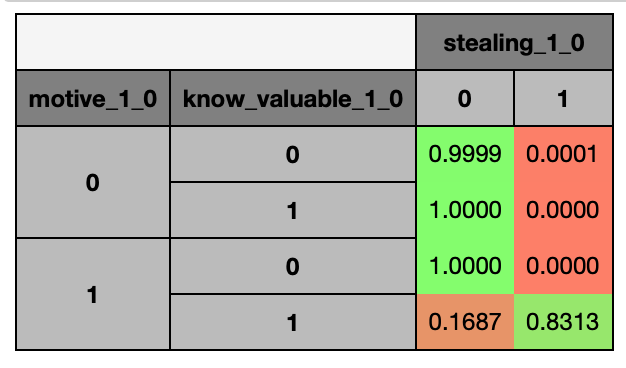
\includegraphics[width=0.6\linewidth]{images/cptStealing.png}
\caption{ Conditional probability table for `stealing\_1\_0'.}
\label{cptstealing}
\end{figure}%

\item \textbf{Independent events are not connected to each other.}
The parent node is not conditional on other nodes, which is correct. For the rest of the nodes, the dependency relations are complex.



\end{enumerate}

\subsection{Performance Criteria}
\begin{enumerate}
\item \textbf{Accuracy and RMSE.}

The accuracy of the network is 92.3\%, which is better than in the previous networks. The RMSE is 0.078. 

\item \textbf{Correspondence.}

The frequency of events in the network (without evidence set) correspond to the frequency of events in the simulation within ±0.001, see Table~\ref{testTableGM}.

\begin{table}
\centering
\begin{tabular}{|c|c|c|}
 \hline
 Conclusion & Frequency P(event) & BN P(event)\\
 \hline
seen\_1\_0    & 0.5415& 0.5415\\
know\_valuable\_1\_0  & 0.2285 &  0.2286\\
know\_vulnerable\_1\_0  & 0.5415 &  0.5414\\
motive\_1\_0  & 0.2285 &  0.2285\\
sneak\_1\_0  & 0.2285 & 0.2284\\
stealing\_1\_0  & 0.19 & 0.1900\\
object\_dropped\_accidentally\_0  & 0.1515 & 0.1517 \\
E\_psych\_report\_1\_0  & 0.1815 &  0.1814\\
E\_camera\_1 & 0.999 & 0.9987\\ 
E\_object\_gone\_0  & 0.3415 & 0.3414 \\
E\_camera\_sees\_object\_1\_0  & 0.1890 & 0.1895 \\
 \hline
\end{tabular}
\caption{Do we match with the frequencies?}
\label{testTableGM}
\end{table}


\item \textbf{Sensitivity Values of Output Node.}

In Figure~\ref{sensitivityGM}, we see that in general, all parameters are more sensitive to changes than in the previous network. However, this network remains robust, as the largest sensitivity value that is not the same node, is only 0.45. 

\begin{figure}[htbp]
 \centering
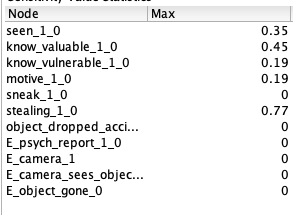
\includegraphics[width=0.6\linewidth]{images/sensitivityGM.png}
\caption{The maximum sensitivity values for every node as it relates to `stealing\_1\_0' as presented in Hugin.}
\label{sensitivityGM}
\end{figure}%


\item \textbf{Evidence updates the posterior in the correct direction.}

We tell the following story with the evidence (Figure~\ref{baseposterior}): We start with no evidence, and a posterior of 0.2 for stealing\_1\_0. This would not be legally correct, before we have any evidence we might have a posterior probability of something being stolen from agent $0$, but we cannot know that it is agent 1 who has done the stealing. In the simulation, where only agent 1 could have stolen the object, it is correct though. Then, we add the evidence that we saw agent 1 on the camera, which is not very strong evidence, because there are a lot of cameras throughout the city. They place the agent at the scene, but are not evidence for stealing. Then, we add the evidence that the object is gone, and the posterior for stealing goes up, but does not saturate to 1, which is also correct - agent 0 could have dropped the object accidentally. Then, we have some evidence of a psychological report, that states that agent 0 fits the victim profile of agent 1, which would be some evidence, but should not be so strong, objectively, as we still have not actually seen any criminal activity from agent 1. Then, finally we see the criminal activity, and see that the camera has seen agent 1 steal the object from agent 0. The posterior for stealing goes to 1.

We note that if we take the same story, but instead of setting `E\_camera\_sees\_object\_1\_0' to 1, we set it to 0, we find P(`stealing\_1\_0) = 0.15, showing both that seeing the thief steal on camera is very strong evidence, and not seeing the thief steal on camera does not mean that they have not stolen (since P(`stealing\_1\_0) $\neq 0$). However, not seeing direct evidence of theft means that the final probability of guilt is too low to convict.

\begin{figure}[htbp]
 \centering
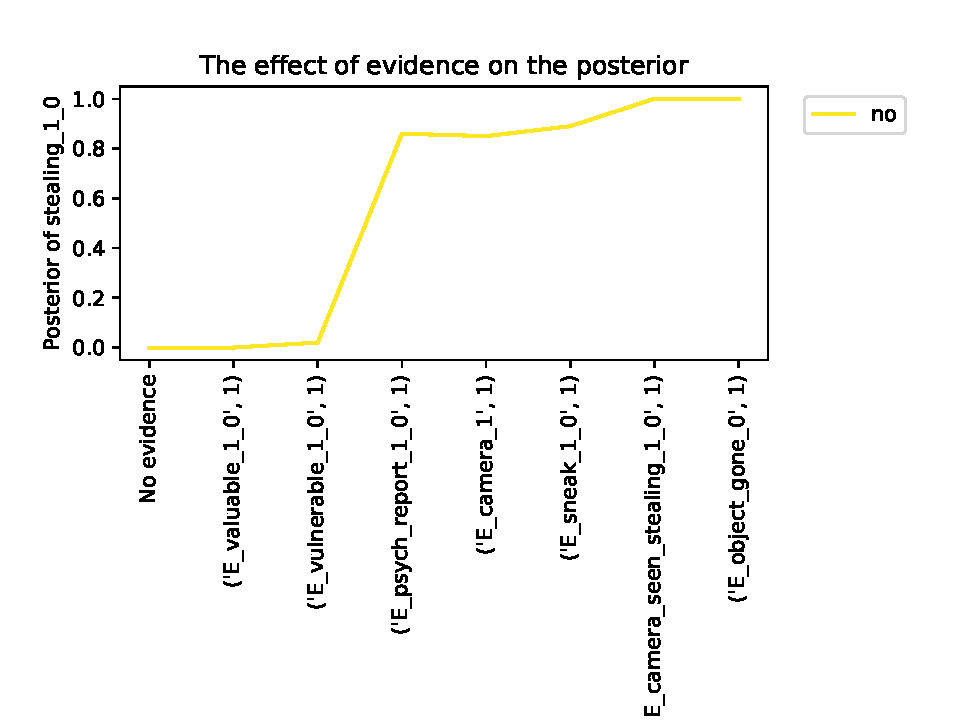
\includegraphics[width=0.6\linewidth]{../experiments/GroteMarkt/plots/posterior_base_networkGroteMarkt.pdf}
\caption{ Progression of evidence resulting in changing the posterior}
\label{baseposterior}
\end{figure}%
\end{enumerate}

\subsection{Human Criteria}
\begin{enumerate}
\item \textbf{How robust is the network against a loss of precision?}

\begin{figure}[htbp]
\begin{center}
\begin{subfigure}{.5\textwidth}
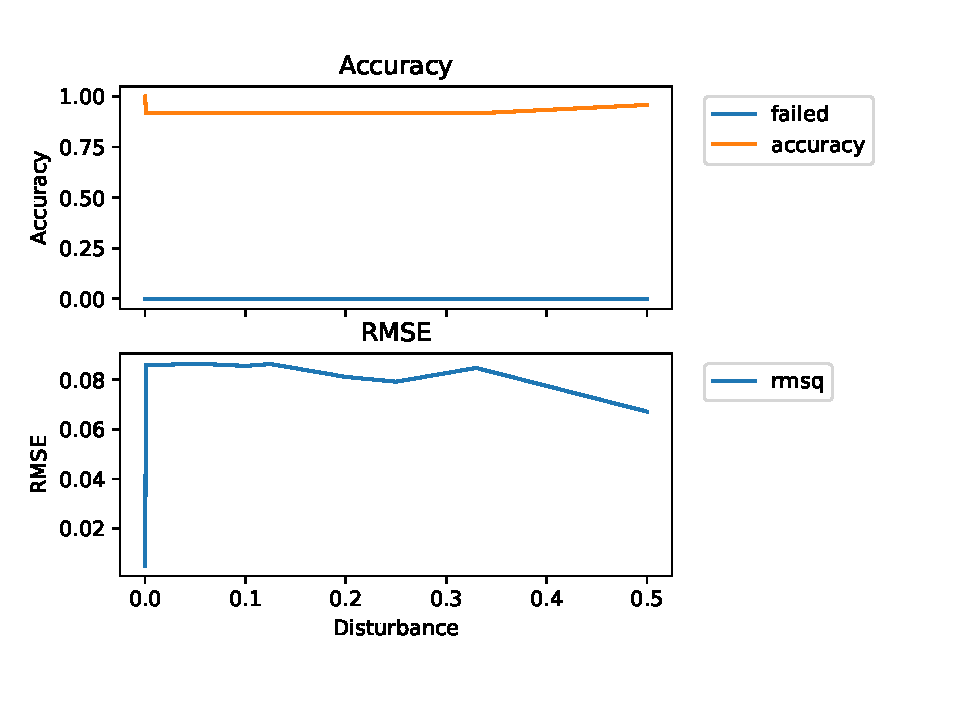
\includegraphics[width=0.9\linewidth]{../experiments/GroteMarkt/plots/performance_GroteMarkt.pdf}
\caption{Network Under Disturbance.}
\label{dist}
\end{subfigure}%
\begin{subfigure}{.5\textwidth}
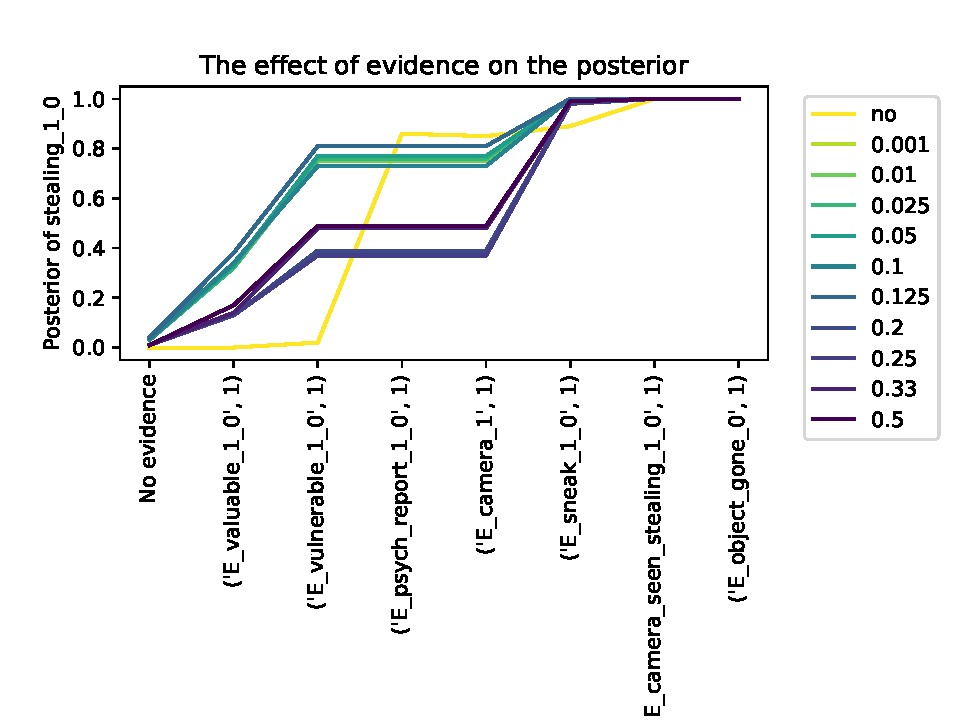
\includegraphics[width=0.9\linewidth]{../experiments/GroteMarkt/plots/posterior_GroteMarkt.pdf}
\caption{ Progression of evidence resulting in changing the posterior}
\label{post}
\end{subfigure}
\end{center}
\caption{Loss of precision in networks.}
\label{pLoss}
\end{figure}

We see again that the networks hold up well against loss of precision (Figure~\ref{pLoss}), which is promising for human builders, as long as they do not assign 1 and 0 but instead $1 - \epsilon$ and $\epsilon$.

\item \textbf{Could a person find these probabilities?}

Since the accuracy of the network does not suffer much under lack of precision, we have more room for error. However, it remains unclear how the probabilities should be determined. For instance, the node `object\_dropped\_accidentally\_0', has a posterior probability of 0.15 when no evidence is added (and two parents). This posterior probability emerges from the in-fact parameter that at any time step before reaching the goal state, the victim has a 1/500 chance of dropping the object. The time before the victim reaches the goal state depends on the victim's initial location and their goal state, both of which are random at every new iteration of the simulation. This means that it would be very difficult to trace this frequency of 0.15 back to factors that can meaningfully be elicited.

On the other hand, nodes like `motive' are almost constructed logically (Figure~\ref{cptmotive}), which implies that we might not need to elicit probabilistic information about all hypotheses nodes - if we find appropriate priors for nodes without parents, and their children can be constructed out of logical combinations of their parents, we might only need to elicit probabilistic information for the parents. However, most of the hypothesis nodes are not such logical combinations, and hence need effortful and almost impossible-to-find information about frequencies.

\begin{figure}[htbp]
 \centering
 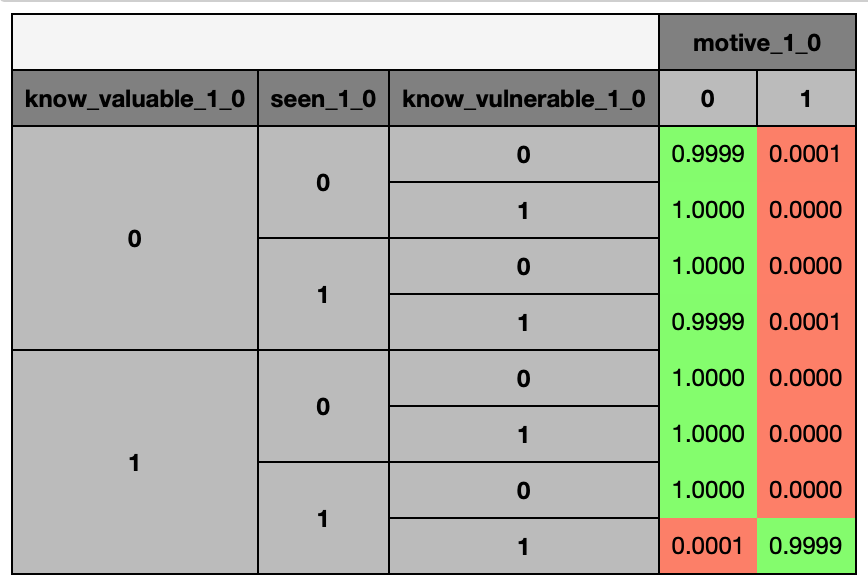
\includegraphics[width=0.6\linewidth]{images/cptMotive.png}
\caption{ Conditional probability table for `motive\_1\_0'. A logical approach.}
\label{cptmotive}
\end{figure}%

\item \textbf{Can a person determine the correct independence relations?}

The network has more dependence relations than would be ideal for a person to create. The ordering of the nodes would be plausible, but there are too many independence relations: `know\_valuable\_1\_0' has 5 children! That is not necessary, it should only have `know\_vulnerable\_1\_0' and 'motive\_1\_0' as children.

\end{enumerate}


\section{Discussion}

We have shown in this chapter that we can generate satisfactory Bayesian Networks from simple agent-simulations with non-trivial environments. These networks can be used to reason towards a conclusion about a posterior probability, given a set of evidence. The network is accurate and is robust under imprecision. However, there are too many arcs in the network, and it is unclear how we should elicit the correct probabilities.

\subsection{Limitations of the simulation.}
This simulation should be seen as a preliminary for further research, as it is lacking in several aspects: the environment is still too simple, the agent-behaviour is too static, and there are only two agents in the simulation. These are the same weaknesses as identified in \citep{Zhu2021}. Expanding the simulation to include or improve these aspects is useful for future research.

The non-trivial environment is still not reflecting the non-trivialness of real environments. The environment of a city offers different affordances to different people, but here the map is shared by all agents. Additionally, shops and buildings can actually be entered.

There is a lack of dynamic behaviour in the agents. They can move around and decide to steal from someone, but they do so based on simple factors. This does not meaningfully reflect the real dynamics of street crime - for example, the vulnerable agent walks around with their valuable object in plain sight, why would they do that if they know that there are thieves on the loose?

One of the purposes of modelling a `real' location is to model the people within that real location. There are many people around on the Grote Markt in real life, modelling just two of them (and not modelling interactions with the crowd) is sufficient to show that automated Bayesian Networks might work in this situation. However, situations where Bayesian Networks might rely on statistical data from real samples (that might be taken from real locations, like the Island Prior), are not modelled in this simulation. 

\subsection{The problem of identity}
We have avoided the problem of identity in this network, because we only have two agents, and one of the agents is always the thief, the other the victim. As soon as we create a more plausible simulation of crime, where everyone could, in principle, rob everyone, given the right incentives, we would need a different kind of reporter. Even if we created the same simulation, but now the victim agent might also be able to rob the thief-agent, we would need twice the amount of nodes (we need `stealing\_0\_1', and the rest as well). Three agents that can each rob each other, and we have 6 times as many nodes, resulting in for $n$ agents, $n(n-1)$ number of nodes if we use the same structure. This is very implausible due to complexity constraints. However, generalising the nodes (so using `stealing', instead of `stealing\_0\_1') means that we have to represent the identity of the suspect in some other way. It is unclear how that is to be done.


\subsection{Implicit conditioning on environment}

We used one non-trivial environment to create this network. However, the underlying geometry of the simulation affects the probabilities that can be found in the simulation. We cannot just assume one prior probability for `seen\_1\_0', since the probability whether some agent sees the other, depends on the structure of the environment. We can show this by using the exact same agent behaviour, but placing the agents on a different map.

Instead of the Grote Markt, we selected 5 different parts of Groningen (Figure~\ref{maps}), converted them into maps according to the method, and then let the agents loose in them to rob each other.
\begin{figure}[htbp]
\begin{center}
\begin{subfigure}{.5\textwidth}
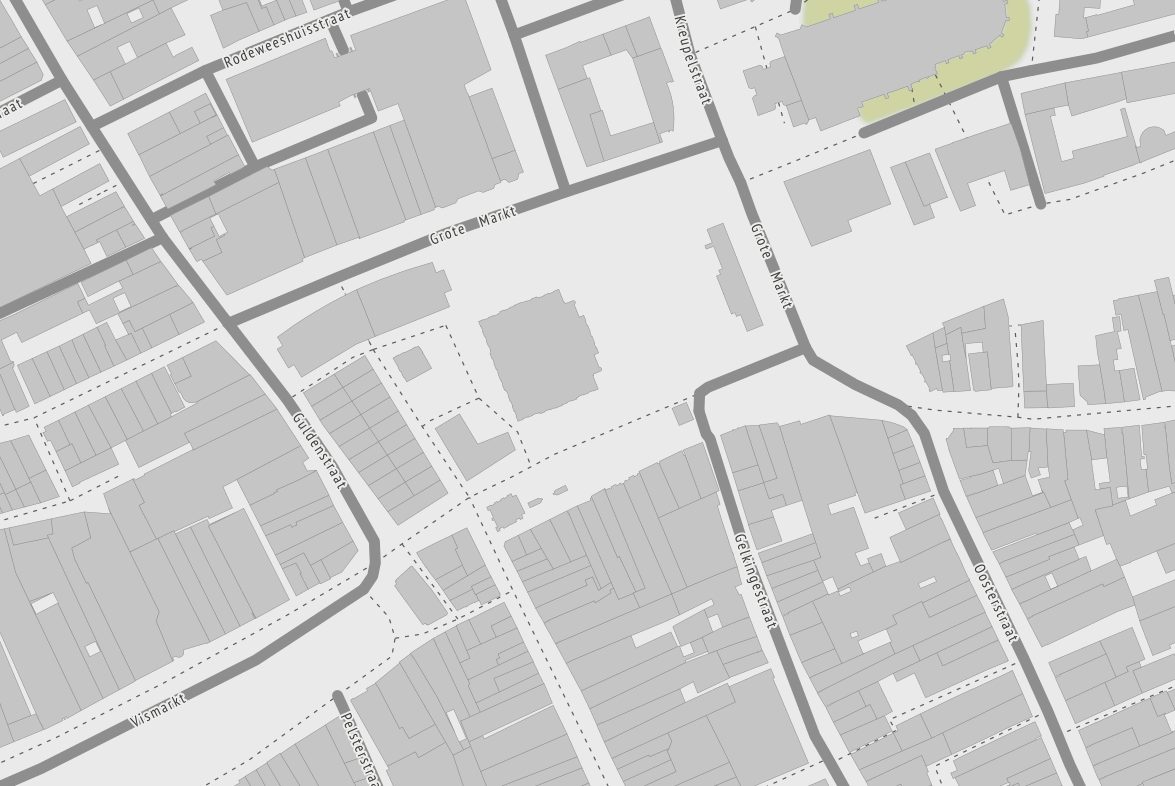
\includegraphics[width=0.8\linewidth]{../experiments/GroteMarktMaps/maps/groteMarkt.png}
\caption{Grote Markt.}
\end{subfigure}%
\begin{subfigure}{.5\textwidth}
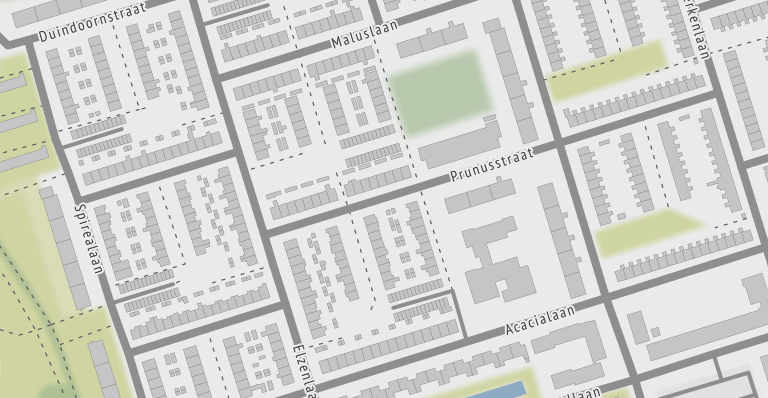
\includegraphics[width=0.8\linewidth]{../experiments/GroteMarktMaps/maps/Selwerd.png}
\caption{Selwerd.}
\end{subfigure}
\begin{subfigure}{.5\textwidth}
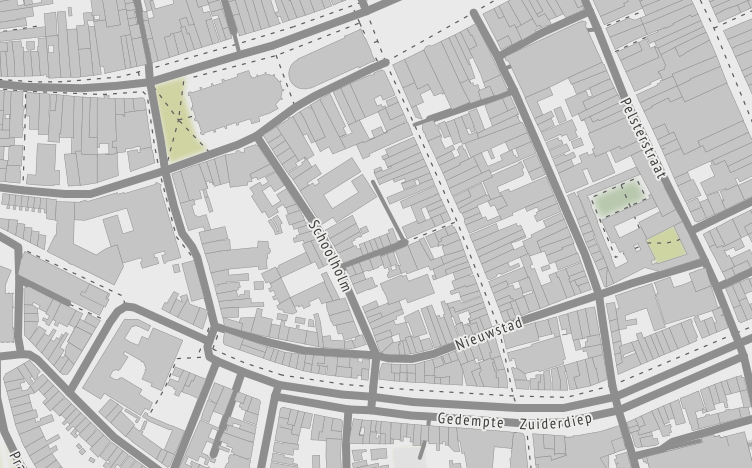
\includegraphics[width=0.8\linewidth]{../experiments/GroteMarktMaps/maps/zuidCentrum.png}
\caption{South-center}
\end{subfigure}%
\begin{subfigure}{.5\textwidth}
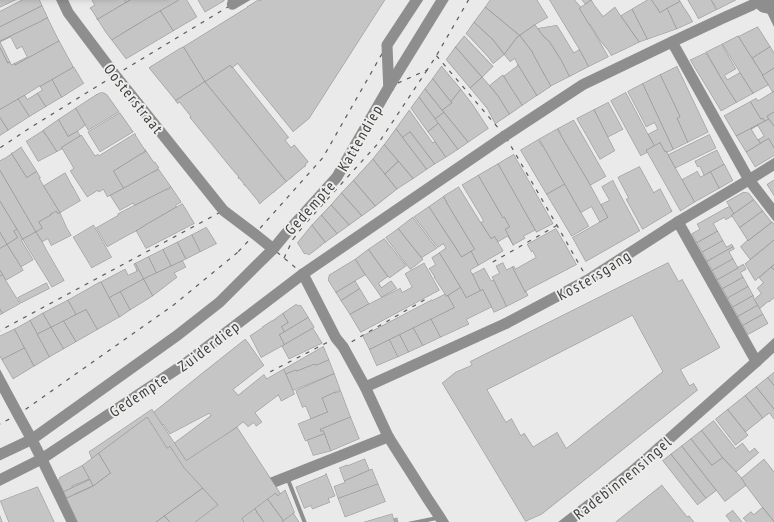
\includegraphics[width=0.8\linewidth]{../experiments/GroteMarktMaps/maps/kattediep.png}
\caption{Kattediep}
\end{subfigure}
\begin{subfigure}{.5\textwidth}
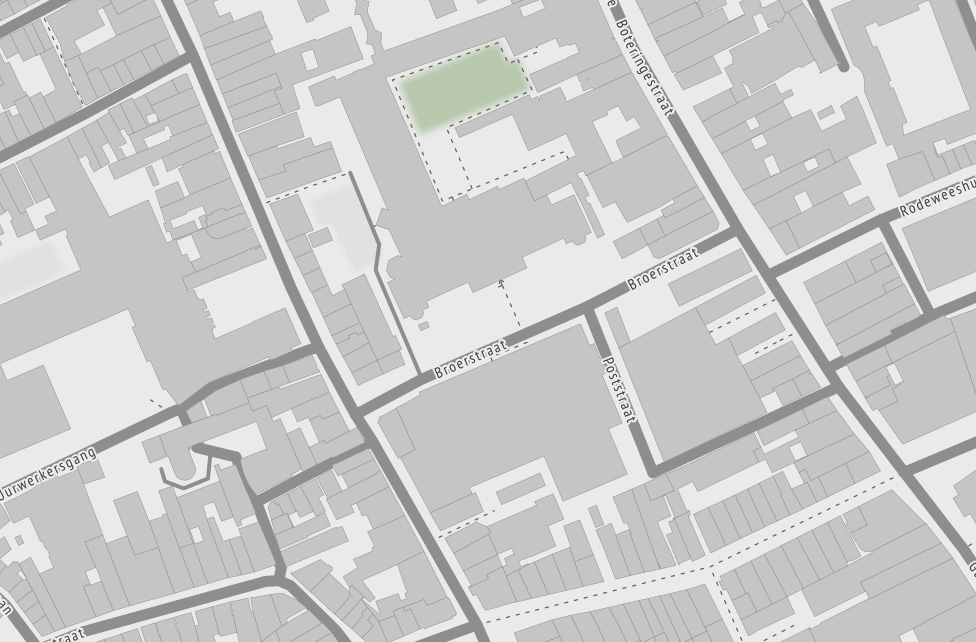
\includegraphics[width=0.8\linewidth]{../experiments/GroteMarktMaps/maps/academy.png}
\caption{Street with the academy building}
\end{subfigure}%
\begin{subfigure}{.5\textwidth}

\includegraphics[width=0.8\linewidth]{../experiments/GroteMarktMaps/maps/wall.png}
\caption{Not Groningen, just a wall}
\end{subfigure}
\caption{Maps.}
\label{maps}
\end{center}
\end{figure}


We look at the difference in the cpt tables for `seen\_1\_0', which represents the event that agent 1 (the thief), sees agent 0 (Table~\ref{mapstab}). If we did not need to condition on underlying geometry of the simulation, we would expect that this probability of `seen\_1\_0' would be the same, regardless of map. However, we find that the probability of the thief seeing the potential victim, depends on the underlying map. 

This means that we actually cannot speak of just one `global' probability for `seen\_1\_0'. The probability of the thief seeing the victim depends on a variable that is not included in the Bayesian Network: the map. Instead of a `global' probability for `seen\_1\_0', that applies to all maps, we can only speak of the probability of the agent seeing the victim as conditioned on a specific map. 

Implications of this is that we need to condition explicitly on maps for our networks to work, because it does meaningfully change the probabilities that we find. Additionally, there's no way to predict how the map that we're using affects the probability of `seen\_1\_0', this probability emerges from the interaction of the agents with the map. This has implications for the real world, because it means that we can't depend on some generic ``probability of getting robbed'', we need to condition on spatial conditions, and background world assumptions.

\begin{table}[htbp]
\begin{tabular}{lllll}
map & accuracy & cpt of `seen\_1\_0' True \\
\hline
selwerd& 1 & 0.471\\
academy & 0.92 & 0.951\\
groteMarkt & 1 & 0.534\\
kattediep & 1 & 0.534\\
wall & 1 & 0.512\\
zuidCentrum &1 & 0.509\\
\end{tabular}
\caption{Difference in cpt depending only on difference in underlying map, no further difference in agent behaviour!}
\label{mapstab}
\end{table}



\subsection{Possible Legal Interpretations.}

As we found in the network in the previous chapter, the problem of operationalisation continues to haunt us. The simulation has very clear operationalisation, as represented by the always-correct reporters. However, it is unclear what shape these reporters should take outside of our simulation. Lawyers and judges would have to ask themselves the following questions, to be applied to every node:

\begin{itemize}
\item \textbf{By what method can we find out whether this event happened or not?}

This question can be answered relatively easily for evidence nodes. For instance, we would know that `E\_camera\_1' would be true in real life, if we saw agent 1 on a relevant camera. For our psychological report, we would know that this event did not happen if the psychiatrist decided that the victim did not fit the suspect's profile.

However, this becomes very complex for hypothesis nodes. How would you find out of `stealing\_1\_0' is true in real life? In our simulation, we just set the event to 1 if it happened. In real life, how would you operationalise this? It is unclear. Should we decide that `stealing\_1\_0' is true if the victim says that their object was stolen? That's perhaps a part of an operationalisation, but it is not a completely valid one, since we know that people can lie about their stuff being stolen. If we say, the victim should say that their object was stolen, and we should find the object on the thief, we are still in trouble if the thief decides to sell the object before they can be apprehended. What would be the method to find out that the state of the real world is such that you could say that `stealing\_1\_0' is true, or false?

 In the real world, we do not need an operationalisation for these kinds of facts, because we all `sort of know what we mean'. However, in Bayesian Networks we need an operationalisation, because Bayesian Networks and random variables are mathematical objects, and need to map events to truth values. This cannot be done without operationalisation.

\item \textbf{If we have a method, how do we decide which events we want to include in our frequency calculation?}

This is the problem of the reference class. To take the example of camera, if we include all cameras in the inner city, the probability that the thief would be seen is great, and hence would not be very relevant to proving the thief's guilt. However, if we decide that we will only use cameras that were on the victim's trajectory, we have limited the amount of cameras, and the probability of the thief showing up on one of these `coincidentally' is lower, hence it would be a stronger piece of evidence if we found that it was true (and more exculpatory if we found that it was false). 

Even though the reference class is a fundamental problem, as long as every legal participant is aware of it, and can argue about why some reference class is better than another class, or decides on the appropriate classes together, this should not be a limiting factor for the Bayesian Network in itself. However, it requires a great deal of work that would not be done if Bayesian Networks were not used, and it is unsure if it would actually result in better outcomes.

\end{itemize}

These essential questions should come before talking about Bayesian Network accuracy, precision or structure, especially if these networks are to be used for practical applications.
